\documentclass[a4paper, landscape]{article}

\usepackage[utf8]{inputenc}
\usepackage[DIV=13]{typearea}
\usepackage{microtype}
\usepackage{mathtools, amssymb, bm}
\usepackage{parskip}
\usepackage[shortlabels]{enumitem}
\usepackage{graphicx}
\usepackage{subcaption}
\usepackage{float}
\usepackage[colorlinks=true]{hyperref}
\hypersetup{linktoc=all}

\title{6}
\date{} 

\begin{document}
\maketitle
\section{Implementation Details}
Note that we have assumed that the angles are drawn uniformly at random from $0$ to $180$ degrees. With this, we don't have to take account the reverse projection vectors as they are just usual projection vectors for some angle in the above range.

For a fair comparison, angles of larger $N$ cases contain the angles of smaller $N$ case. In other words, each increment in value of $N$ can be observed as adding more angles to smaller values cases

To get the reconstructed images with same orientation as the original image, first reflect the reconstructed image (if applicable) and then rotate the resulting image clockwise by the provided angle.
\section{Observations}
\begin{itemize}
	\item In \ref{fig:ri}, reconstructions have good enough detail with more than $500$ angles also evident by decreasing RMSE with increasing $N$ (0.32 to 0.18)
	\item In \ref{fig:rif} with $100$ angles, minimum RMSE value of the rotated output image with the original image is in the same orientation as the original image
\end{itemize}
\begin{figure}[H]
	\centering
	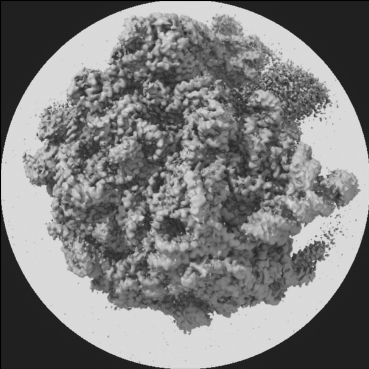
\includegraphics[width=0.2\linewidth]{results/cryoem.png}
	\caption{Original Image}
	\label{fig:oi}
\end{figure}
\begin{figure}[H]
	\centering
	\begin{subfigure}{0.13\linewidth}
		\centering
		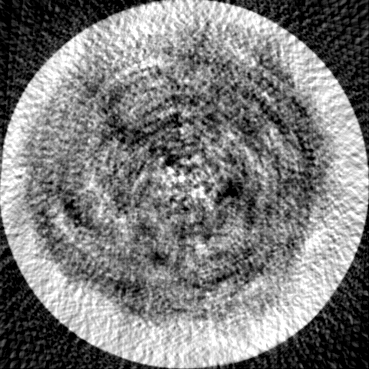
\includegraphics[width=\linewidth]{results/cryoem, N = 50.png}
		\caption{$(50, 0.31731)$}
	\end{subfigure}
	\begin{subfigure}{0.13\linewidth}
		\centering
		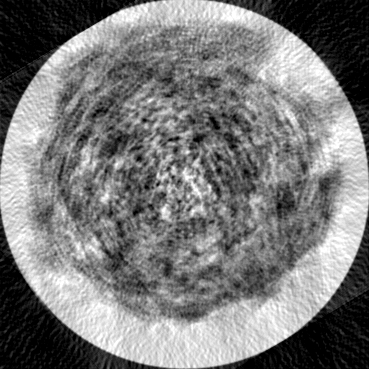
\includegraphics[width=\linewidth]{results/cryoem, N = 100.png}
		\caption{$(100, 0.25435)$}
	\end{subfigure}
	\begin{subfigure}{0.13\linewidth}
		\centering
		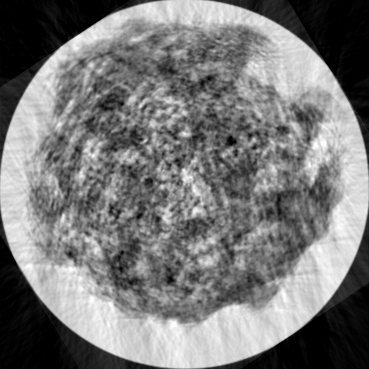
\includegraphics[width=\linewidth]{results/cryoem, N = 500.png}
		\caption{$(500, 0.2102)$}
	\end{subfigure}
	\begin{subfigure}{0.13\linewidth}
		\centering
		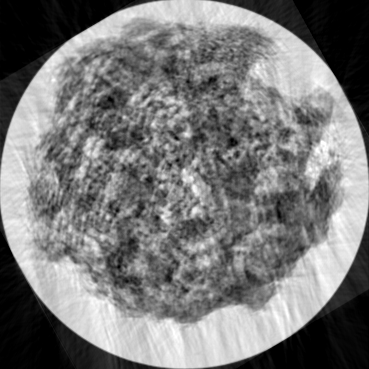
\includegraphics[width=\linewidth]{results/cryoem, N = 1000.png}
		\caption{$(1000, 0.19902)$}
	\end{subfigure}
	\begin{subfigure}{0.13\linewidth}
		\centering
		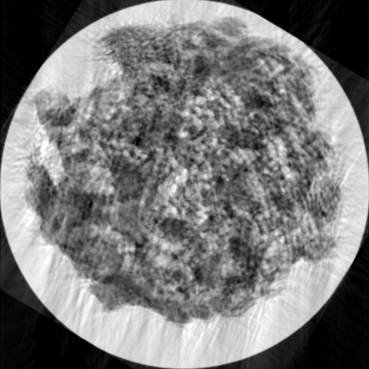
\includegraphics[width=\linewidth]{results/cryoem, N = 2000.png}
		\caption{$(2000, 0.19149)$}
	\end{subfigure}
	\begin{subfigure}{0.13\linewidth}
		\centering
		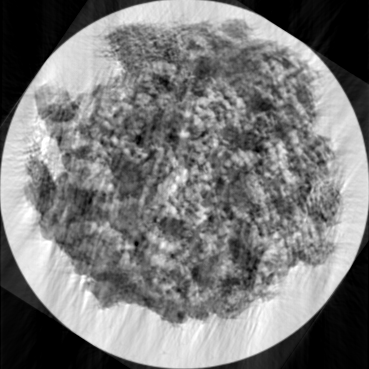
\includegraphics[width=\linewidth]{results/cryoem, N = 5000.png}
		\caption{$(5000, 0.1835)$}
	\end{subfigure}
	\begin{subfigure}{0.13\linewidth}
		\centering
		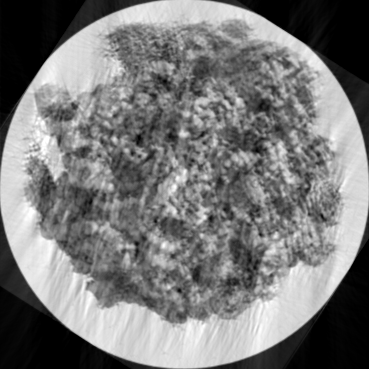
\includegraphics[width=\linewidth]{results/cryoem, N = 10000.png}
		\caption{$(10000, 0.17778)$}
	\end{subfigure}
	\caption{Reconstructed Images, with $(N, \text{RMSE})$}
	\label{fig:ri}
\end{figure}
\begin{figure}[H]
	\centering
	\begin{subfigure}{0.13\linewidth}
		\centering
		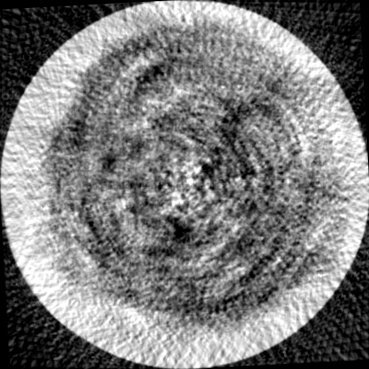
\includegraphics[width=\linewidth]{results/cryoem, N = 50 and rotated by angle = 87.png}
		\caption{$(50, 87^\circ, \text{no})$}
	\end{subfigure}
	\begin{subfigure}{0.13\linewidth}
		\centering
		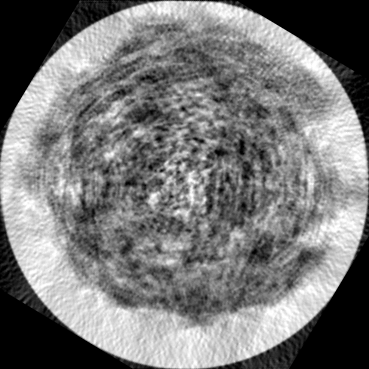
\includegraphics[width=\linewidth]{results/cryoem, N = 100 and rotated by angle = 31.png}
		\caption{$(100, 31^\circ, \text{no})$}
	\end{subfigure}
	\begin{subfigure}{0.13\linewidth}
		\centering
		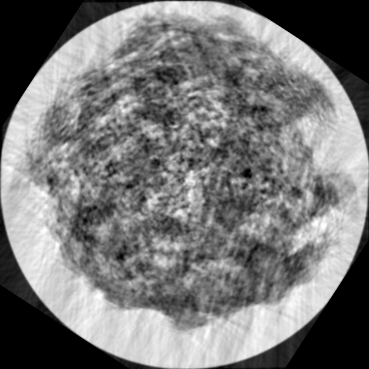
\includegraphics[width=\linewidth]{results/cryoem, N = 500 and rotated by angle = 33.png}
		\caption{$(500, 33^\circ, \text{no})$}
	\end{subfigure}
	\begin{subfigure}{0.13\linewidth}
		\centering
		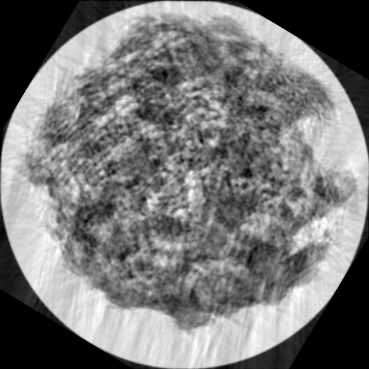
\includegraphics[width=\linewidth]{results/cryoem, N = 1000 and rotated by angle = 31.png}
		\caption{$(1000, 31^\circ, \text{no})$}
	\end{subfigure}
	\begin{subfigure}{0.13\linewidth}
		\centering
		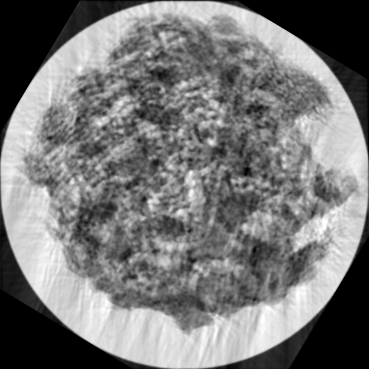
\includegraphics[width=\linewidth]{results/cryoem, N = 2000, reflected and rotated by angle = 31.png}
		\caption{$(2000, 31^\circ, \text{yes})$}
	\end{subfigure}
	\begin{subfigure}{0.13\linewidth}
		\centering
		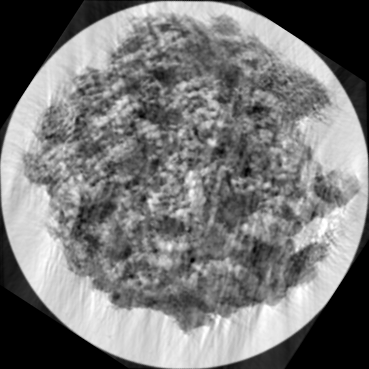
\includegraphics[width=\linewidth]{results/cryoem, N = 5000, reflected and rotated by angle = 33.png}
		\caption{$(5000, 33^\circ, \text{yes})$}
	\end{subfigure}
	\begin{subfigure}{0.13\linewidth}
		\centering
		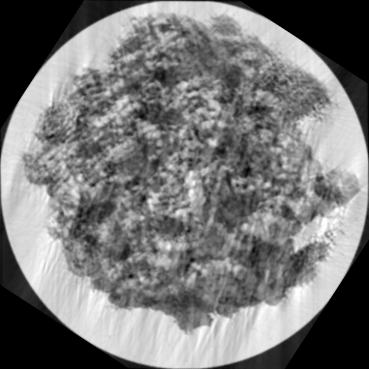
\includegraphics[width=\linewidth]{results/cryoem, N = 10000, reflected and rotated by angle = 33.png}
		\caption{$(10000, 33^\circ, \text{yes})$}
	\end{subfigure}
	\caption{Reconstructed Images with approriate RMSE minimising rotation (clockwise) with(out) reflection $(N, \text{angle, reflected?})$}
	\label{fig:rif}
\end{figure}
\end{document}